\documentclass[english]{ccdconf}
\begin{document}


\title{3D Object Detection in RGBD Image Using View Independent Feature}
\author{Jiang Liu\aref{sjtu}, Jianxun Li\aref{sjtu2}}

\affiliation[sjtu]{School of Electronic Information and Electrical Engineering,
Shanghai Jiao Tong University, Shanghai, 200240
        \email{jiangliux@sjtu.edu.cn}}


\affiliation[sjtu2]{School of Electronic Information and Electrical Engineering,
	Shanghai Jiao Tong University, Shanghai, 200240
	\email{lijx@sjtu.edu.cn}}

\maketitle

\begin{abstract}
These instructions give you basic guidelines for preparing papers
for Chinese Control and Decision Conference . Note that ``Abstract''
and ``Key Words'' are bold.
\end{abstract}

\keywords{Paper, Instruction, Chinese Control and Decision
Conference }

\footnotetext{This work is supported by National Nature Science
Foundation under Grant ********.}

\section{INTRODUCTION}

%Object detection has received considerable attention recently. It consists of two key tasks: (\romannumeral1) object categorization which determines if any instance of the categories of interest presents in a given image, and (\romannumeral2) object localization which estimates the positions and extents of detected objects.
3D object detection has received considerable attention recently for the wide range of applications in autonomous driving and personal robotics\cite{xiang2014beyond}. Traditional detection method only localize objects in 2D bounding boxes, missing the information of 3D location, orientation and 3D extent. In contrast, 3D object detection provide accurate 3D information to understand real world, thus plays an important role in morden computer vision.\\
It is difficult to solve this task in RGB image due to its natrual ambiguity of missing depth. The most common approach is to discretize the viewing sphere into bins and train a 2D detector for each viewpoint \cite{gu2010discriminative}. However, only weak 3D information can be obtained in these methods. Besides, object-centerd methods establishes spatial connections betwee views by mapping them directly to the surface of 3D model. Though these types of models seems attractive for the continuous viewpoint represantations, their detection performance has typically been inferior to 2D deformable models. More recently, \cite{fidler20123d} extend 2D deformable part-based models(DPMs)\cite{felzenszwalb2010object} to 3D space by means of a deformable 3D cuboid.\\
With the the availability of inexpensive RGB-D sensors, such as Microsoft Kinect, Apple PrimeSense, Intel RealSense, and Google Project Tango, larger and more ambitious RGBD datasets are created which enabled major breakthroughs for highlevel scene understanding\cite{silberman2012indoor,janoch2013category}. SUN RGB-D dataset\cite{song2015sun}, which contains 10,335 RGB-D images with dense annotations in 3D, has become a de-facto standard for scene understanding.\\
It is important to exploit the depth information to advance 3D object detection. Sliding Shapes\cite{song2014sliding} was proposed to slide a 3D detection window in 3D space, detect objects by matching to CAD models in “sliding” locations. While CAD models can potentially provide abundant information, the number of models for all categories is limited, and thus this method focused only on a small number of categories. Ren\cite{ren2016three} proposed the Clouds of Oriented Gradients(COG) feature that links the 2D appearance and 3D pose of object categories. COG accurately describes the 3D appearance of objects with complex 3D geometry.\\
Our contribution are two folds:
first, Instead of scanning every possible location and orientation in 3D space, we use rectified 3D Selective Search to dramaticlly speed up the testing process with a relative high recall. 
second, object pruning is uesed to reduce candidate object hypothesis in testing stage, thus reduce testing time as well as false positive detection.
\section{Related Work}

\subsection{3D Feature}
The histogram of oriented gradient (HOG) descriptor \cite{dalal2005histograms} is widely used in object detection. Basiclly, it counts occurrences of gradient orientation in localized portions of an image, and its performance is good enough for 2D detection.  However, since gradient orientations are determined by 3D object orientation and perspective projection, HOG descriptors that are naively extracted in 2D image coordinates is not suitable for 3D object description.\\
To handle this issue, many work has been done. some used extra CAD model to describe the edge from various viewpoints\cite{aubry2014seeing}.Other assumed that object in sepecific views are near-planar\cite{fidler20123d}. previous extensions of the HOG descriptor  to 3D space require full mesh model\cite{buch20093d}. The cloud of oriented gradient(COG) feature, without all these assumption, accurately model the 3D apperence of objects.\\
Like HOG , the calculation of COG can be divided into 3 step: Gradient computation, 3D orientation bin construction and normalization. In the first step, gradient of the image is computed by applying filters [-1,0,1], [-1,0,1]$^\mathrm{T}$ to RGB channels. Gradient in position $(x,y)$ is obtained by setting  maximum responses across
color channels to $(dx,dy)$, with corresponding magnitude $\sqrt{(dx^2+dy^2)}$.
Then, cuboid contains the object is devided it into $6\times6\times6$ voxels, and 9 orientation bins are constructed for each voxel to model the distribution of local 3D gradient orientation. Perspective projection is used to find corresponding 2D bin boundaries. For each point lies in a voxel, its projected gradient magnitude is sumed into corresponding 2D orientation bin, which is back-projected into 3D bin. Last, bilinearly interpolation is performed between neighboring bins.
 Histogram $\phi_{il}^c$for voxel $l$ in cuboid $i$ is normalized by setting $\phi_{il}^c \leftarrow \phi_{il}^c / \sqrt{\|\phi_{il}^c \|^2+ \epsilon}$ for a small $\epsilon>0$, so the dimension of COG feature is a fixed size of $6^3\times9=1944$.

\subsection{3D Search}
Search algorithm define the hypothesis space for potention object location in testing image. Sliding window method is widely used in 2D detection algorithm\cite{dalal2005histograms,felzenszwalb2010object} and the core idea is intuitive.  An exhaustive search with predefined step is performed where all the location within the image is scanned to not miss any potential object location. Scale is considered by examined different size of image patch at that location. However, searching all the possible location is computationally expensive. Selective search is proposed for fast computation with high recall\cite{uijlings2013selective}. First, initial regions is obtained by performing fast segmentation\cite{felzenszwalb2004efficient}. Later, the most similar neighbouring region pair is merged into a new region and add to the set in every iteration. Finally, object location boxes are extracted from all regions in the set.\\
The current search methods in 3D naively generlized from 2D. Sliding shape\cite{song2014sliding} train an Exemplar-SVM on a CG model rendered at a specific 3D location relative to the virtual camera, then perform exhaust search only at the nearby location of the CG model in order to improve the speed. This 3D local search approach results a relative low recall rate. In \cite{ren2016three}, 3D space is discritized into grids. The at each possible location, certain size of bounding boxes which based on the empirical statistics of trainning bounding boxes, along with 16 candidate orientation are examined. This strategy brings a high recall rate but introduce many false positive detection.\\
3D selective search(3D SS) is first  proposed in \cite{kanezaki20153d}. But it finally outputs candidate bounding boxes in 2D image. \cite{song2016deep} rectified this method and output 3D bounding boxes. First, RANSAC is used to fit the pane of 3D point cloud to obtain an initial segmentation. For each plane that its projection covers more than 10\% of the total image area,
RGB-D UCM segmentation from \cite{gupta2014learning}(with threshold 0.2) is used for further splitting. Then starting with this oversegmentation, different segmentation regions are hierarchically grouped, with the following similarity measures:
\begin{itemize}
\item $s_{color}(r_i,r_j)$ is the measurment of color similarity between region $r_i$ and $r_j$ using RGB color histogram intersection.
\item $s_{\#pixels}(r_i,r_j)=1-\frac{\#pixels(r_i)+\#pixels(r_j)}{\#pixels(im)}$, where $\#pixels(\cdot)$ is number of pixels in this region.
\item
$s_{volume}(r_i,r_j)=1-\frac{volume(r_i)+volume(r_j)}{volume(room)}$, where $volume(\cdot)$ is the volume of 3D bounding boxes of the points in this region.
\item
$s_{fill}(r_i,r_j)=1-\frac{volume(r_i)+volume(r_j)}{volume(r_i \cup r_j)}$ describe how well region $r_i$ and $r_j$ fit into each other.
\end{itemize}
The weighted sum of these four terms form the final output of similarity measuremenmt. Since both 3D and color cues are combined,
this very strong baseline achieves an average recall 74.2\%.
\section{PIPELINE}
During trainning(Sec. \ref{Train}), we learn a structred svm for each class with COG combined with geometry features, without the extra information of CG model. During testing(Sec. \ref{Test}), we use learned structured SVMs to classify candidate cuboids produced by improved 3D Selective Search method, and output 3D bounding boxes with detection scores.
\subsection{Trainning}
\label{Train}
\subsection{Testing}
\label{Test}
\section{EVALUATION}
\section{CONCULUSION}
%\subsection{Instructions for Authors}
%
%In order for the proceedings to be ready for distribution at the
%conference, an electronic copy (PDF format) of the final version of
%your paper must be submitted via CCDC Paper Management System via
%\URL{http://www.ccdc.neu.edu.cn/}. Please follow the submission
%instructions shown on the web site.

%\section{FORMATTING INSTRUCTIONS}
%
%\LaTeXe{} Authors: please try to use the paragraph styles contained
%in this document.
%
%\subsection{Length}
%
%The maximum allowed number of pages is 6.
%
%\subsection{Page/Font Settings}
%
%It is strongly recommended that prospective authors download
%suitable style file for use with \LaTeX{} and templates for use with
%MS Word.
%
%Style files and templates provided here have been created to ensure
%that margin requirement is adequately met. If, for some reason, you
%are not able to use provided templates or style files, please
%observe the following margins and font settings strictly.
%
%%\begin{table}
%%  \centering
%%  \caption{Page Margins}
%%  \label{tab1}
%%  \begin{tabular}{l|l}
%%    \hhline
%%    Paper Size          & (21$\times$29.7)cm \\ \hline
%%    Top Margin (1st page)   & 3.5cm \\ \hline
%%    Top Margin (rest)   & 2cm \\ \hline
%%    Left Margin         & 1.9cm \\ \hline
%%    Right Margin        & 1.9cm \\ \hline
%%    Bottom Margin       & 2.7cm \\ \hline
%%    Text Width          & 17.2cm \\ \hline
%%    Text Height         & 25cm \\ \hline
%%    Column Width        & 8.25cm \\ \hline
%%    Column Separation       & 0.7cm \\
%%    \hhline
%%  \end{tabular}
%%\end{table}
%
%%\begin{table}
%%  \centering
%%  \caption{Font Settings}
%%  \label{tab2}
%%  \begin{tabular}{c|c}
%%    \hhline
%%    Title           & Times New Roman, 16pt,bold \\ \hline
%%    Author List         & Times New Roman, 11pt \\ \hline
%%    Authors�� Address       & 9pt \\ \hline
%%    Abstract, Key Words     & 9pt \\ \hline
%%    Section Titles      & 11pt,bold \\ \hline
%%    Subsection Titles       & 10pt,bold \\ \hline
%%    Normal Text         & 10pt \\ \hline
%%    Table/Figure Captions   & 9pt \\ \hline
%%    References, Footnotes   & 8pt \\
%%    \hhline
%%  \end{tabular}
%%\end{table}
%
%\subsection{Section and Subsection Headings}
%
%Number section and subsection headings consecutively in Arabic numbers and
%type them in bold. Avoid using too many capital letters. If any further
%subdivision of a subsection is needed the titles should be 10 point and
%flushed left.
%
%\subsection{Main Text}
%
%Use Times New Roman with font size 10 point for text (character
%size). Paragraphs are separated by 6 point and with no indentation.
%You may type on plain white A4 paper. Typing area should not exceed
%172mm${}\times{}$250mm. The text should be prepared with a double
%column format and single line spacing.
%
%\subsection{Tables}
%
%All tables must be centered in the column and numbered consecutively
%(in Arabic numbers). Table headings should be placed above the table.
%Place tables as close as possible to where they are mentioned in the
%main text (see Table~\ref{tab1} and Table~\ref{tab2}).
%
%\subsection{Figures}
%
%All illustrations should be original drawings or photographic prints of
%originals.  Photographs should be glossy prints. Photocopies are often
%not good enough and should be avoided.  All illustrations must be numbered
%consecutively, using Arabic numbers.  Center figure captions beneath the
%figure (see Figure~\ref{fig1}). If possible, do not assemble figures at the
%back of your article, but place them as close as possible to where they are
%mentioned in the main text. No part of a figure should go beyond the typing
%area. Captions should appear below graphical objects, as in Figure~\ref{fig1}.
%
%\begin{figure}
%  \centering
%  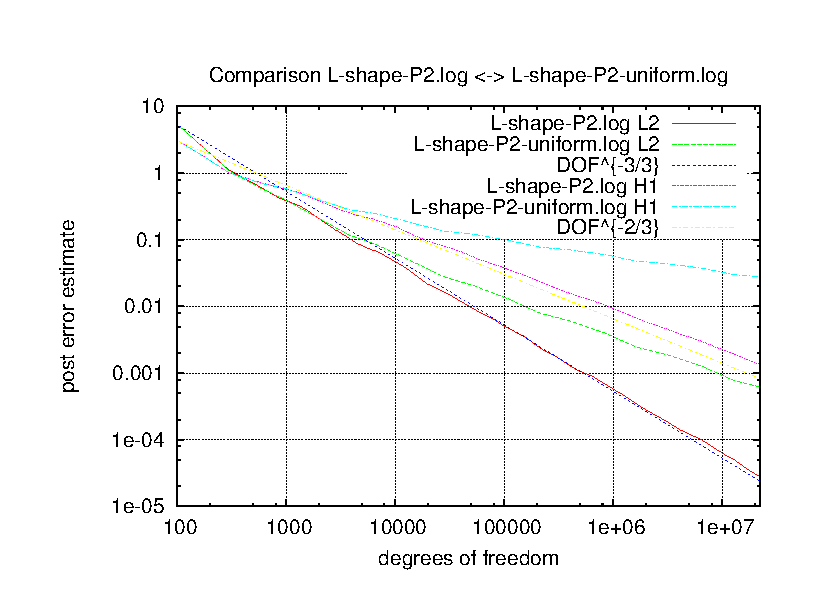
\includegraphics[width=\hsize]{fig1.eps}
%  \caption{The Caption}
%  \label{fig1}
%\end{figure}
%
%Color and grayscale figures should be prepared with 400 dpi
%resolution and  saved with no compression, monochrome figure should
%be prepared with 600 dpi resolution and saved with no compression.
%
%\subsection{Mathematical Formulas}
%
%Mathematical formulas should be roughly centered and have to be numbered
%as formula~(\ref{eq1}).
%\begin{equation}
%  \label{eq1}
%  \lambda_{1,2} = 0.5 \left[\, c_{11} + c_{12}
%            \sqrt{(c_{11} + c_{12})^2 + 4 c_{12} c_{21}} \,\right]
%\end{equation}
%
%\subsection{References}
%
%Number citations consecutively in square brackets \cite{bib1}. The
%sentence punctuation follows the brackets \cite{bib3}. Please note
%that the references at the end of this document are in the preferred
%referencing style. Give all authors's names; do not use ``et al.''
%unless there are six authors or more. Use a space after authors'
%initials.
%
%%
%% Note: place a \balance command somewhere within the left column of the
%% last page will balance the two columns on the last page.
%%
%\balance
%
%\section{CHECKLIST}
%
%\begin{itemize}
%  \item Do not end a page with a section or subsection heading.
%  \item Do not include page numbers in the text.
%  \item Large figures, tables and mathematical equations may span both columns.
%  \item To balance the two columns on the last page, place the command
%    \verb|\balance| somewhere in the text of what would be the first
%    column of the last page without balanced columns.
%  \item If you have to plug a large formula, table, etc.,  which needs a cross
%  column space, you must add option \verb|usemulticol| into the
%  commend \verb|\documentclass|, then use the commend
%  \verb|\singlecolumn{content}| to input cross column contents.
%
%
%\end{itemize}

%\section{PAPER SUBMISSION}
%
%After proofreading your paper, it (PDF formats) must be submitted
%via \URL{http://www.ccdc.neu.edu.cn/}.\cite{fidler20123d}


%\begin{thebibliography}{0}
%
%\bibitem{bib1}D. Z. Cheng, Controllability of switched  bilinear systems, IEEE
%Trans. on Automatic Control, Vol.50, No.4, 511-515, 2005.
%%----------the format for published papers-----------------
%
%\bibitem{bib3} H. Poor, An Introduction to Signal Detection and
%Estimation,   New York: Springer-Verlag, Chap. 4, 1985.
%%--------- the format for books-------------------------
%
%\bibitem{bib4} B. Smith, An approach to graphs of linear forms, accepted.
%
%\end{thebibliography}

\bibliographystyle{ieeetr}
\bibliography{pol}

\end{document}
